
%\section{The Leap Motion Controller}
The latest technological breakthrough in gesture-sensing devices has come in the form of a Leap Motion Controller (Leap Motion, San Francisco, CA, United States). 
The controller, approximately the size of a box of matches, allows for the precise and fluid tracking of multiple hands, fingers, and small objects in free space with 
sub-millimeter accuracy~\citep{Guna2014}.

\section{Physical properties}
The Leap Motion Controller (see fig. \ref{fig:leapmotion} and \ref{fig:leapmotion2}) contains two stereoscopic cameras, with a field of view of about 150 degrees, 
in addition to three infrared LEDs. These infrared lights periodically emit light pulses with a wavelength of 850 nanometer, and thus outside the visible light spectrum. 
During the light pulses, 
which light up about eight cubic feet in front of the controller, grayscale stereo images are captured by the cameras and sent to the 
Leap Motion tracking software~\citep{LeapMotion2016}. 
This image capturing has an effective range from approximately 25 to 600 millimeters above the device.
In the software, the images are analyzed to reconstruct a 3D representation of what the device sees, 
compensating for static background objects and ambient environmental lighting. 
The Leap Motion software combines this sensor data with an internal model of the human hand to help cope with challenging tracking conditions.


\begin{figure}%[h!] %[H]
	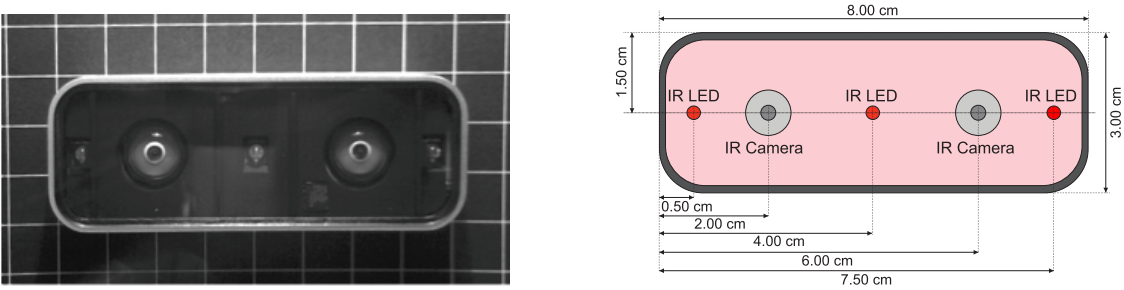
\includegraphics[width=\linewidth]{pictures/LMC_measures.png}
	\caption[Visualization of a Leap Motion Controller]{Visualization of a Leap Motion Controller, with Infrared Imaging (left) and a Schematic View (right)~\citep{Weichert2013}.}
	\label{fig:leapmotion2}
\end{figure} 

\section{The Leap API}
The controller itself can be accessed and programmed through high level Application Programming Interfaces (APIs), with support for a variety of programming languages, 
including C++, C\#, Objective-C, Java, JavaScript and Python. Although the API is programmed almost exclusively in C, access through a variety of other languages 
is achieved by virtue of various "wrapper libraries", which exposes and translates functions from their respective languages into the corresponding C function[cite].
In addition to this, the Leap Motion SDK also features integration with commercial game engines such as Unity and the Unreal Engine~\citep{Guna2014}. 
This section will cover important concepts in the Leap API, which are thoroughly used in the thesis implementation.

\begin{figure}%[h!] %[H]
	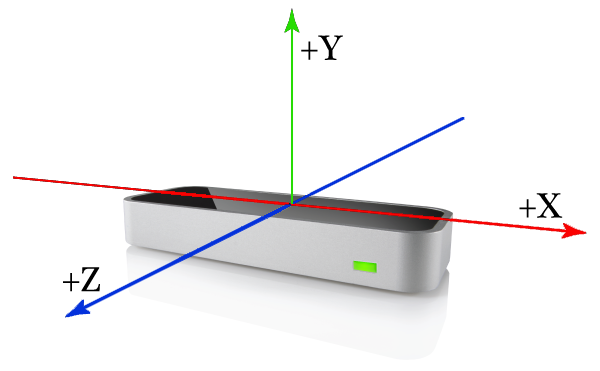
\includegraphics[width=\linewidth]{pictures/Leap_Axes.png}
	\caption[Leap Motion Coordinates]{The Leap Motion Coordinate System has its origin between the two cameras.}
	\label{fig:leapmotion3}
\end{figure} 

\subsection{The coordinate system}
The Leap Motion API enables acquisition of the recognized object's position through Cartesian and spherical coordinate systems, 
which are used to describe positions in the controller's sensory space~\citep{Guna2014}. The hand positions above the Leap Motion device are given as three dimensional
vectors on the form {x, y, z}, with origin being in the center of the Leap Motion surface (see \ref{fig:leapmotion3})~\citep{LeapMotion2016}.  
Positional information, like the position of a hand, or the position of the tip of a finger, can be access in various ways. One way is to access the
"Frame-object", which is an object-oriented representation of the last captured frame of the device. This object exposes functions and variables like
"hands" to get access to an object representation of each hand present in that frame. Each hand-object also have an object-representation of its fingers, its palm
etc, where the positional coordinates for this entities can be acquired individually. Below is an example of this in C\#:

\lstset{style=csharp}
\begin{lstlisting}
using UnityEngine;
using System.Collections.Generic;
using Leap;

public class LeapBehavior : MonoBehaviour {
    LeapProvider provider;

    void Start ()
    {
        provider = FindObjectOfType<LeapProvider>() as LeapProvider;
    }

    void Update ()
    {
        Frame frame = provider.CurrentFrame;
        foreach (Hand hand in frame.Hands)
        {
          if (hand.IsLeft)
          {
              transform.position = hand.PalmPosition.ToVector3() +
                                   hand.PalmNormal.ToVector3() *
                                  (transform.localScale.y * .5f + .02f);
              transform.rotation = hand.Basis.Rotation();
          }
       }
    }
}
\end{lstlisting}

The Leap Motion API uses a right-handed coordinate convention, meaning that when the user is positioned in front of the Leap Motion Controller the x-axis grows more positive 
towards the right, the y-axis grows more positive upwards and the z-axis grows more positive towards the user (see \ref{fig:leapmotion3}). 
As frameworks like that of Unity uses a left-handed convention for its coordinate system, i.e that the z-axis grows more positive away from the 
user instead of towards, the Leap Motion API also does an appropriate convention to adhere to its software environment. 
The Leap Motion API also adhere to differences in units, as e.g Unity uses a default unit of meters, while the Leap Motion uses millimeters~\citep{LeapMotion2016}.


\subsection{The detection utilities}


% Technically, very few details are publicly known about the precise nature of the algorithms used due to patent and trade secret restrictions.

\section{Important Leap components}




% Hands, fingers, palm, directions, frames, interaction box etc. 
% See \\
% https://developer.leapmotion.com/documentation/csharp/devguide/Leap\_Overview.html\#motion-tracking-data \\
% https://developer.leapmotion.com/documentation/csharp/devguide/Leap\_Coordinate\_Mapping.html\#map3d \\
% https://developer.leapmotion.com/documentation/csharp/devguide/Leap\_Hand.html \\


\section{Detectors - The building blocks of gesture recognition}
The detector scripts. How they can be combined. Logic gates. 
% See https://developer.leapmotion.com/documentation/unity/unity/Unity\_DetectionUtilities.html

\section{Integration with the Unity editor}
How the pieced fit together. How the stuff is organized (e.g the modules).
% See https://developer.leapmotion.com/documentation/unity/index.html